\chapter{Data Preprocessing \& \\System Architecture}
\label{pp_sa}

Section \ref{data_pp} gives an overview of how input data was pre-processed.
Section \ref{architecture} describes the technical set up required for running all these experiments and deploying the model to production.

\section{Data Preprocessing}
\label{data_pp}

There were around a dozen product features that affiliate networks provided.
Most of these were either categorical or textual,  with just a single numerical feature.
Initially, the data was analysed using Dataprep, a Google Cloud Platform (GCP)  product for data wrangling, which at the time of use was in beta stage.
Dataprep  was used to process a sample of ~800 000 products;  it produced histograms of the values present in each feature column (see figure \ref{dataprep}).

\begin{figure}
 \hspace*{-0.2\textwidth}
 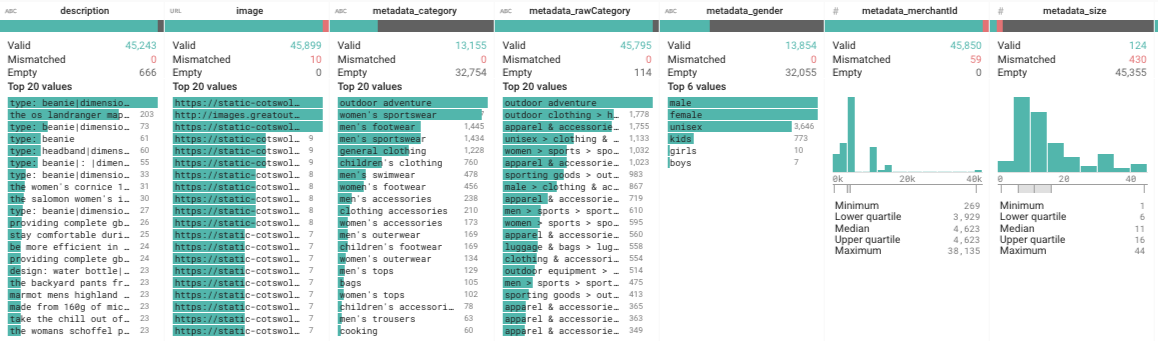
\includegraphics[width=1.4\textwidth]{figures/dataprep}
 \caption{Dataprep: the histograms of field values of a subset of fields.}
 \label{dataprep}
\end{figure}


The histograms revealed that a lot of the input features were mostly empty, but also that many of the inputs that would naturally be considered categorical  had much more unique value in them then one might expect.
For example, each affiliate gives us the textual representation what they consider to be the category of the product,  but  rather than containing a small number of unique tokens, these contained all the full category paths along with the category delimiters, which  varied retailer by retailer (e.g.  it was common to see both ``Shoes > Sneakers'' and ``Shoes // Sneakers'').
Representing these as categorical variables would have blown up the input space, which would have  resulted in more parameters, each parameter having fewer examples to learn from.
Therefore, many such ``categorical''  were actually represented as text, which were tokenised and cleaned appropriately, allowing for better generalisation and smaller models.

There was a single numerical field: price.
This could have been min-max normalised to the range 0 ... 1, however there  was a small number of very high values that would have squash nearly all the other  prices.
Rather than  carefully considering  how to mitigate this,  the input dimension was dropped, because it is not likely to have much predictive value for product classification.
It would be trivial to bring this feature back for a training objective for which it would be much more useful.

A trickier question was how many distinct tokens or categorical values to keep per input column.
Keeping all of them would not have been sensible: there were still large numbers of tokens that appeared only once, often because there were some unwanted formatting characters, misspellings, or incorrect punctuation that caused a token to be considered a separate entity.
There was a single configuration file that dictated which models used which features as input, whether those inputs were represented as textual, categorical, or dense values;  it also determined  the maximum number of unique values/tokens,  and the dimensionality of the embedding.
This configuration file was read by Dataflow during pre-processing  and by TensorFlow during  inference and training, which made experimentation with  different types of models and input representations considerably easier.

Below is a list of input features with information about how they were represented; it also lists the dimensionality of embeddings  for the models which  encoded categorical variables as embedding.

\begin{itemize}[noitemsep]
 \item title - text - max 8000 unique tokens
 \item brand - categorical - max 5000 unique values - 10 embedding dimensions
 \item category - categorical - max 950 unique values - 6 embedding dimensions
 \item rawCategory - text - max 1000 unique tokens
 \item description - text - max 8000 unique tokens
 \item gender - categorical - take all unique tokens
 \item size - categorical - max 100 unique tokens
 \item image - dense vector of 2048 or 1280 dimensions extracted with a 2D CNN
\end{itemize}


\section{System Architecture}
\label{architecture}

 The following technologies were used to build the system which had to interact with existing services  at the client company:

\begin{itemize}
  \item Apache Airflow (AF) - a Python framework for defining workflows of long-running tasks and dependencies between these tasks.
  \item TensorFlow (TF) - ML framework for Python, capable of defining many kinds of models as a computation graph, and executing this graph locally or in a distributed manner.
  \item ML Engine (MLE) - a GCP service for running TensorFlow models (training, hyperparameter tuning, inference).
  \item Apache Beam - a data processing engine akin akin to Apache Spark.
  \item Dataflow - a GCP service for executing Apache Beam workloads.
  \item Tensorflow Transform - a Python library with a small set of operations for data preprocessing that can run inside a TensorFlow graph as well as an Apache Beam pipeline.
  \item Google Cloud Storage (GCS) - Google Cloud Platform (GCP) object storage similar to Amazon S3.
  \item ElasticSearch (ES) - a NoSQL database with powerful full-text search and querying capabilities.
  \item RabbitMQ - a message queue, used for transferring data among our microservices (using the Logstash adapter, that can read from and write to (among other things) ElasticSearch and RabbitMQ).
  \item Flask - a simple backend web framework for Python.
  \item Node.js - a JavaScript backend web framework.
  \item React.js - a JavaScript front-end framework for JavaScript.
  \item Redux - a framework for persisting user interface (UI) state and application data in single page applications.
  \item GraphQL - a query language for building flexible APIs
\end{itemize}

Figure \ref{arch_diagram} shows the how data is passed between the main services, and how services and technologies interact.

All product data is stored in ElasticSearch (ES): the labels, top predictions of the ML system, and evaluation metrics from various train runs.
ES is accessed from the public web application via GraphQL and the ML administration web UI (further referred to just as web UI\footnote{The web UI was initially built with Flask and React by the author as a quick way to get insight about the model, and then re-written as a more feature-rich version by an employee of the client company with Node.js, GraphQL, React and Redux.}).
Data is pulled into the ML pipelines by dumping the results of an ES query to a local file, which is uploaded to GCS.
Updates to the ES index are not done directly, since indexing the updated products is computationally expensive; instead, updates are put on a RabbitMQ queue, which is consumed by Logstash, which in turn updates products in ES at a rate that will not overburden the servers.

All ML training and prediction happens in a batch-oriented way, encapsulated as Airflow pipelines.
Each pipeline is a directed acyclic graph of tasks, where a task can be a shell command or Python function; a pipeline defines dependencies of task execution, which allows us co-ordinate a series of operations that could be executed locally (inside the Docker container running AF) or remotely (such as in a GCP service).
A typical pipeline dumps data locally, uploads it to GCS, schedules a Dataflow job to preprocess data, polls the Dataflow service until the Dataflow job is finished, schedules an ML engine job, polls the MLE service until it has completed, and runs an update process that reads the predictions and evaluation statistics from GCS and sends the updates to the RabbitMQ queue.
Reading updates and sending these to RabbitMQ is done in a parallelised manner (using multiprocessing), since the update process is bottlenecked by network latency as well as computing the appropriate category path for each product (explained in \ref{cat_tree}).

\begin{figure}
  \hspace*{-0.2\textwidth}
  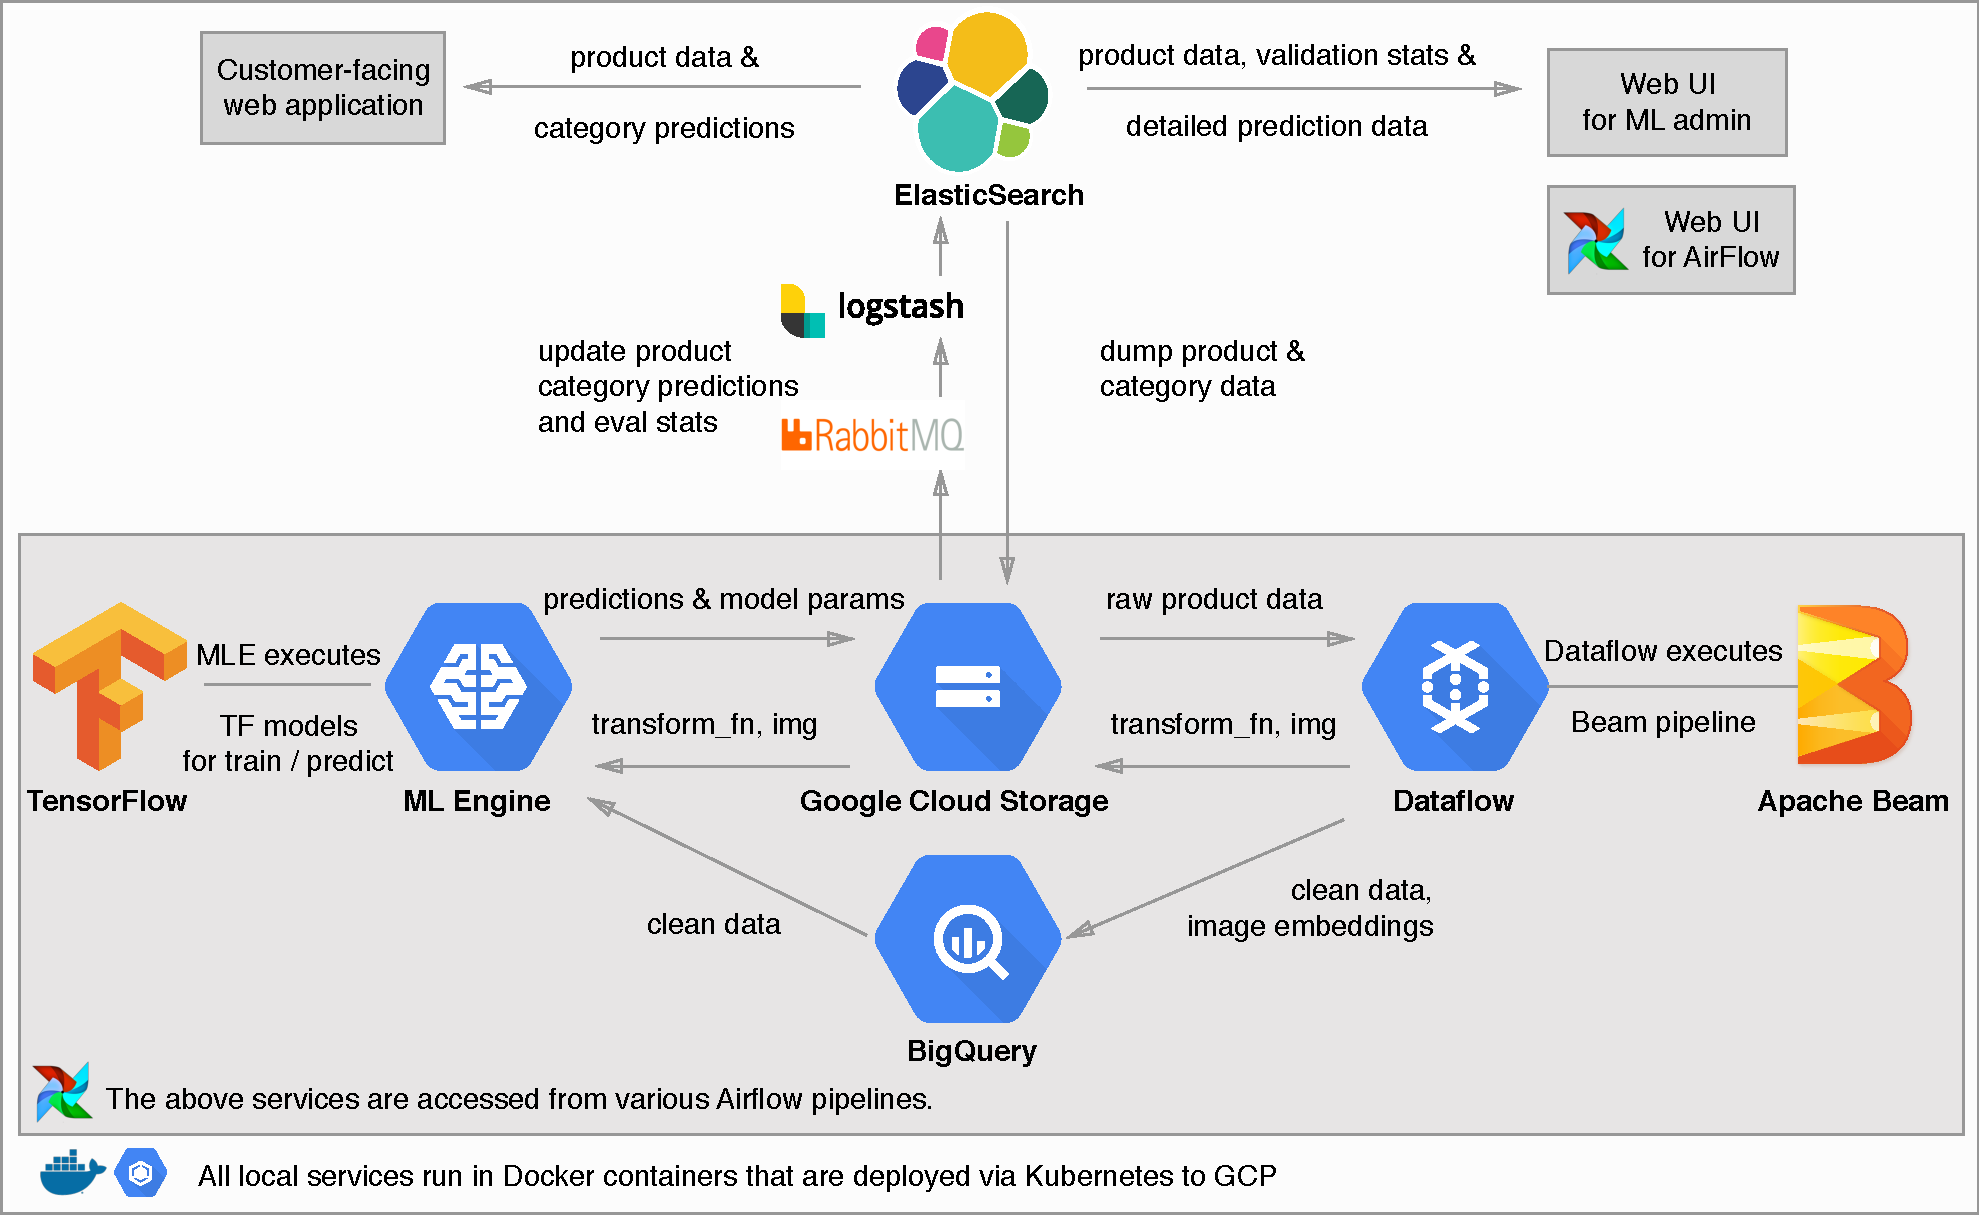
\includegraphics[width=1.4\textwidth]{diagrams/architecture}
  \caption{High-level system architecture of the ML pipeline}
  \label{arch_diagram}
\end{figure}

\subsection{Airflow Pipelines \& Pipeline Runs}

A group of tasks that would need to be run together repeatedly is encapsulated in an Airflow pipeline, which is a directed acyclic graph (DAG) of tasks (also referred to as an AF pipeline).
A DAG is run many times, either based on a schedule or triggered manually.
Figure \ref{fig:af1} shows a screenshot of the most common Airflow pipeline ``cat\_pp\_train\_specific'', which is short for ``categorisation: preprocess and train a specific model''; figure \ref{fig:af2} shows the sub-DAG of the task ``train''.

\begin{figure}
\centering
\begin{minipage}{.48\textwidth}
  \centering
  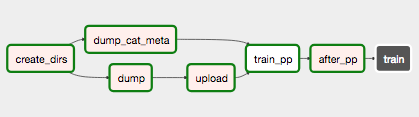
\includegraphics[width=1.0\linewidth]{figures/af_train_specific}
  \captionof{figure}{Airflow DAG: preprocess, train specific model, update statistics. All tasks except for ``train'' have completed, which is not yet scheduled for execution.}
  \label{fig:af1}
\end{minipage}%
\begin{minipage}{.48\textwidth}
  \centering
  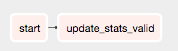
\includegraphics[width=.6\linewidth]{figures/af_train}
  \captionof{figure}{Airflow sub-DAG: train. No task has been scheduled for execution during this run.}
  \label{fig:af2}
\end{minipage}
\end{figure}

Most of our pipelines start by creating directories for our files.
Which files are stored where is configured in a simple file that is accessed by Airflow, Dataflow and TensorFlow (locally or inside MLE); the configuration has placeholders for variables that are determined per run or are specific to a task inside a run.
For example, the location of .tfrecords files is determined by ``\textit{:prefix}/runs/\textit{:run\_id}/ tfrecords/\textit{:objective}\_\textit{:split}.tfrecords'', where \textit{prefix} corresponds to the path to the data directory (either locally or in GCS), \textit{run\_id} is specific to the current run of the pipeline, \textit{objective} is either \textit{rule\_based} or \textit{exclusive}, and \textit{split} is either \textit{train}, \textit{test} or \textit{valid}.
This ensures that all parts of the system look for the same file in the same place, and makes building file paths easier.
All file access in the different parts work equally on a local file system and GCS, which makes it particularly convenient to switch between local experimentation and remote training; in fact, the \textit{prefix} parameter is by default read from an environment variable, which is different in local, Docker and cloud service environments.

A training dataset is identified by its \textit{run\_id}.
The processed .tfrecords, transform function (described below) and metadata is persisted under that run's directory.
Several models can be trained from the same dataset.
The checkpoints of a model are saved under ``\textit{:prefix}/runs/\textit{:run\_id}/checkpoints/\textit{:hparams\_id}/'', where \textit{hparams\_id} identifies a model architecture, as well as what kinds of training objectives and label types it is trained on; during hyperparameter tuning, a unique index is appended to the \textit{hparams\_id} of the model.
As \textit{hparams\_id} encodes only the general model architecture and training objectives, the full set of all hyperparameters is persisted along model checkpoints as a JSON file - for future reference.

\subsection{Dataflow Pipelines}
There are two types of Dataflow pipelines: for preprocessing training data and for calculating product-product visual similarity. Omitting various details, dead-ends and workarounds that were needed due to technical limitations and prior system architecture choices\footnote{which were completely reasonable at the time, when the ML system was not a consideration}, the pipelines had the following tasks:

\subsubsection{Preprocessing}
\label{pp}

This pipeline loads the products dumped from ES (as JSON) and preprocesses data according to a configuration file (see section \ref{data_pp}).
Figure \ref{df} shows a screenshot of this pipeline, as visualised by the GCP UI.

In this pipeline, all fields are cleaned of obvious noise and superfluous whitespace.
Text and categorical fields are tokenised and mapped to integer indices, keeping only the top \textit{k} values and also computing TF-IDF scores for text fields.
This is handled by TensorFlow Transform, which persists this token-to-index mapping in a \textbf{transform function} that is saved to GCS at the end of the pipeline.
The transform function can be used by TensorFlow or Dataflow to convert raw text inputs to a  sparse inputs;
separate pre-processing run will generate a different transform function, with mostly the same tokens mapping to different indices, as the order in which they will be encountered will be different.
The tokenised data is stored to GCS as a sharded .tfrecords files (with one set of files per training objective), a binary file format that TF Transform helps produce; alternatively the raw data could be saved (e.g. as JSON or inside BigQuery) and the transform function inside a TF graph could re-tokenise this raw data at runtime.

\begin{figure}
  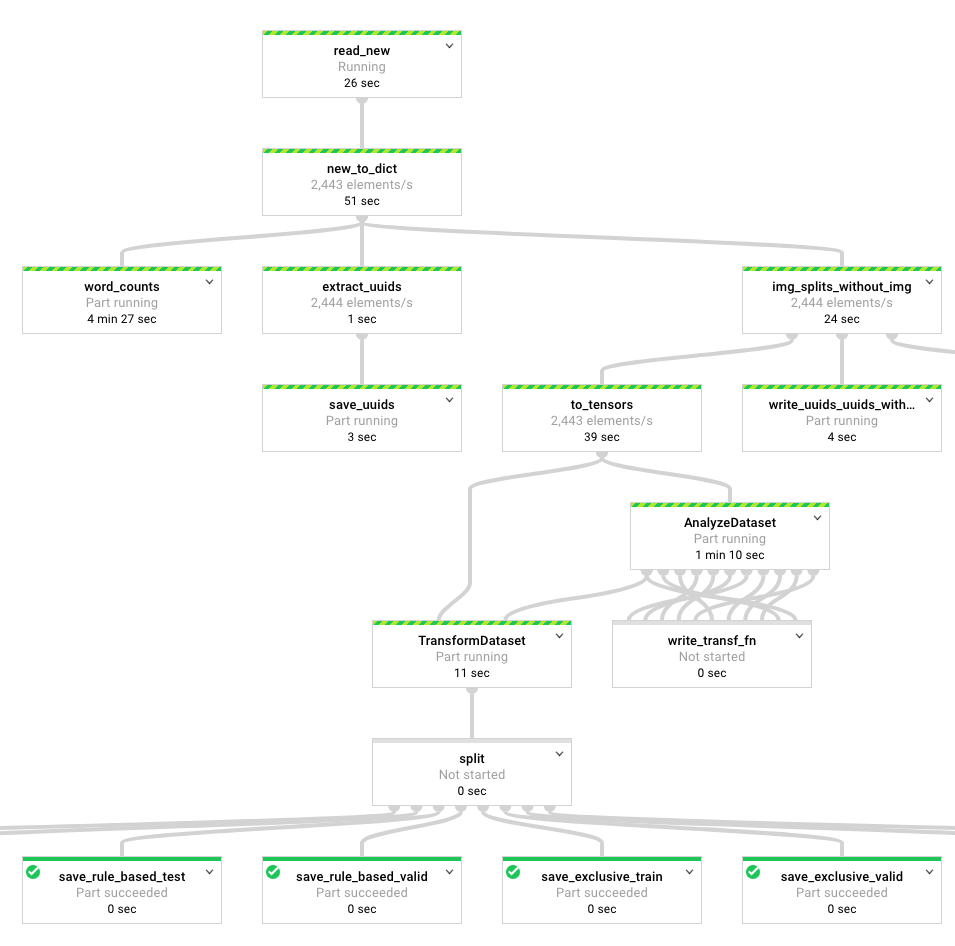
\includegraphics[width=\linewidth]{figures/df}
  \caption{A running Dataflow pipeline of data preprocessing}
  \label{df}
\end{figure}

The pipeline is also responsible for downloading product images, which are saved to GCS as individual files to avoid hitting the content delivery network that stores product images multiple times.
Images are a major bottleneck due to network latency.
To avoid a TF / MLE job from making separate requests to fetch each file individually\footnote{Each request has latency overhead, which compounds quickly when doing million of these.}, Dataflow saves the raw image content into the .tfrecords file; this increases Dataflow execution time, but reduces time and cost overall, as Dataflow is cheaper and easier to parallelise than a MLE job.

A former version of the pipeline also computed image embeddings inside the Dataflow job, but this was inefficient.
We also wanted to have the flexibility to try different models for computing embeddings (e.g. Inception V3, MobileNet, AutoML models) and fine-tuning image models.
Attempts to persist these pre-computed embeddings had severe overheads, and currently the approach is to re-compute these at every time inside MLE, which can leverage a GPU to do it efficiently.

\subsubsection{Visual Similarity}
\label{vis_sim_pp}

The Dataflow pipeline implemented for the experiments described in \ref{exp_sim} relied on image embeddings computed by the preprocessing pipeline.
As explained in section \ref{exp_sim}, it needs to find the \textit{k=100} nearest neighbours of each product based on the cosine similarity of their image embeddings.
The product-product  similarities are the simplest case computed within products that belong to same second level category.
The pipeline read the files output by the preprocessing stage, and partitioned it into datasets by the category predicted in the previous train run, as the new predictions would not be saved in the file.
The per-category image embeddings were merged (using \textit{reduce}) into matrices of image embeddings in a given category, and the top 100 approximate nearest neighbours were extracted for each product using nmslib \cite{nmslib} (as a \textit{map} operation over all the per-category embedding matrices).
The nearest neighbour UUIDs were persisted to GCS and a downstream AF task picked these up and updated ES with these.

This set-up will be replaced in the future.
Computing embeddings in Dataflow is slow, and me way want to enable more flexible ways of restricting the subset of products that are considered (e.g. not just 2nd level category, but a 3rd level category or even globally).
The most flexible approach is one in which nearest neighbours are computed in real time when a product is viewed by a user.
The biggest challenge in such a system is keeping all the image embeddings in memory, which would require 32 GB of memory for the 4 million products we currently have\footnote{$~4000000 * 2048 * 32$ = number of products * embedding dimensionality * 32 bits per number}, and the number of products is likely to increase in the future.

An option worth considering is deploying this as a TensorFlow model to MLE, which reads the embedding matrix in as a sharded tf.Variable; the shards can be distributed on different machines, which is handled automatically by TF.
The input to this model would be just the UUID of the product in question, and the UUID of the category to which the nearest neighbour search is limited; the ``prediction'' of the model would be dot product of the product embedding in question, and all the other product embeddings that are in the given category.
Therefore to get the nearest neighbours of an image embedding, TF would go through all the product embeddings to check for their membership of the given category - but this is fast given all the embeddings are always kept in memory.
The nearest neighbour search will also be precise, which would be prohibitively slow when pre-computing nearest neighbours but should be manageable when done online, as there will be only a handful of requests per second and the dot products are calculated in parallel by multiple workers.
We can also use autoscaling that would increase the number of workers to handle high loads, which would also put all workers to sleep after 15 minutes of inactivity.


\subsection{TensorFlow and ML Engine}

All models were implemented using TensorFlow, using higher level APIs (such as tf.data, tf.estimator and tf.learn) when possible.
This was somewhat challenging, as the high-level APIs were poorly documented, changed even throughout the duration of this project, and it was not clear which APIs are compatible with each other.
Ultimately the only reliable way to understand a class or function was to read its source code.
In many cases these APIs provided almost what was needed, but to support our use case the code was copied from the TensorFlow GitHub repository and adapted to our purpose\footnote{For example, multi-objective learning where each objective potentially changes a subset of the model's variables was not possible due to the way loss from multiple ``heads'' was merged in the current TF APIs. Also some parts had to be rewritten to give us per-class evaluation metrics.}.

The point of entry to the trainer program is the controller.py, which decides based on command line arguments which task to run: train, predict, train and predict, evaluate, export model, etc.
There is a large number of hyperparameters that can be supplied via command-line arguments, with reasonable defaults.

The data was loaded using the tf.data.Dataset API, which provide convenient functions for reading large numbers of files, prefetching, shuffling, batching, and performing arbitrary transformations on the data, such as transforming a set of bytes representing a JPEG image into a 3D tensor of integers.
This works well for simple use cases but is less flexible when for example doing multi-objective learning.
We would like to control roughly how many data points from each objective end up in a batch, or for how long a model is pre-trained on one objective before the second objective is introduced.
Refer to section \ref{multiobj} for a description of two approaches that were tried.
In general, the trainer program would use tf.data.Dataset class to build an \textit{input function} for either training or evaluating, and the input function would be supply data points for the train loop.

TensorFlow models were built using the tf.estimator.Estimator class by providing a custom \textit{model function}.
The model function would dynamically build the model based on the \textit{model type} (deep / linear), \textit{input type} (these are listed in section \ref{exp_models}), \textit{training objectives} and \textit{hyperparameters}.
An input type determines which input features are used and how they are represented, while a training objective determined which training dataset, loss function and evaluation metrics were used.
Both input types and training objectives had simple configuration files dictating their behaviour, which made adding new training objectives and experimenting with different model architectures easy.

Training was handled by the tf.estimator.train\_and\_evaluate function.
It loads a model from the checkpoint directory if present, and trains the model for a specified number of steps, or until the input function terminates.
It also periodically saves model checkpoints to GCS, and handles writing TF summary operations that are needed for data visualisations using TensorBoard\footnote{TensorBoard is a web interface for visualising the variables and metrics a TensorFlow train run produces; many of the visualisations in the following sections are taken from Tensorboard.}
